\subsubsection*{Training Insights}
ResNet101 training was also similar to the other ResNet model's training. Many trainings did not produce good predictions and either suffered from too low mass estimations or other problems due to overfitting. 


\subsubsection*{Best Performing Model}

\begin{figure}[H]
\centering
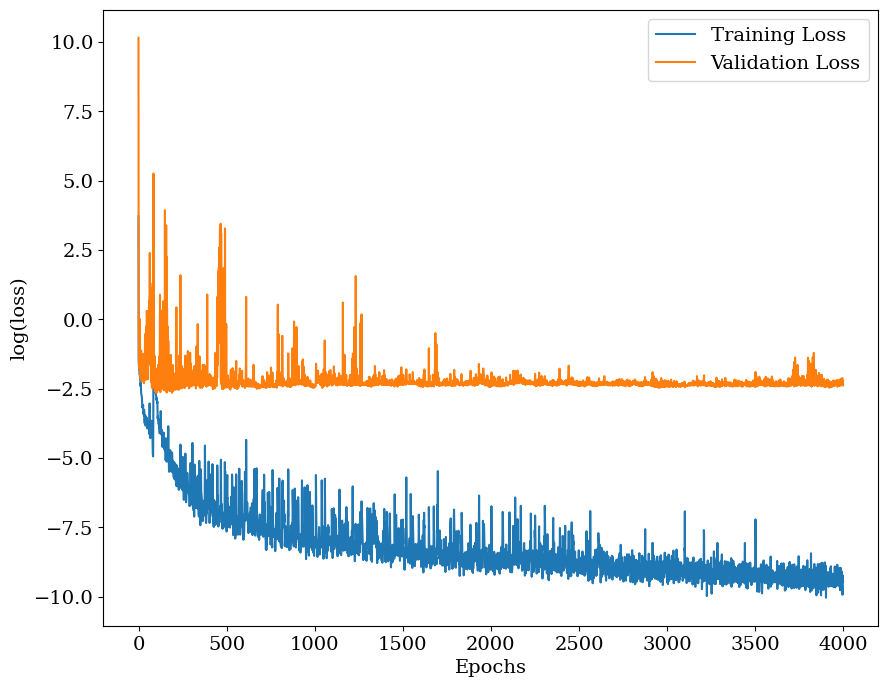
\includegraphics[width=.667\textwidth]{images/Chapter4/Res101/res101_history.png}
\caption{Training history of the best performing ResNet101 model.} 
\label{fig:resnet101_best_history}
\end{figure}

The best ResNet101's training did not have as many spikes in validation loss as many of the other model's training had. The validation loss kept steady after about 1700 epochs of training. After just a few hundred epochs it was at a minimum after which it went up again. This is an indicator for overfitting because the training loss kept on decreasing afterwards. 

\begin{figure}[H]
\centering
\begin{subfigure}{.46\textwidth}
  \centering
  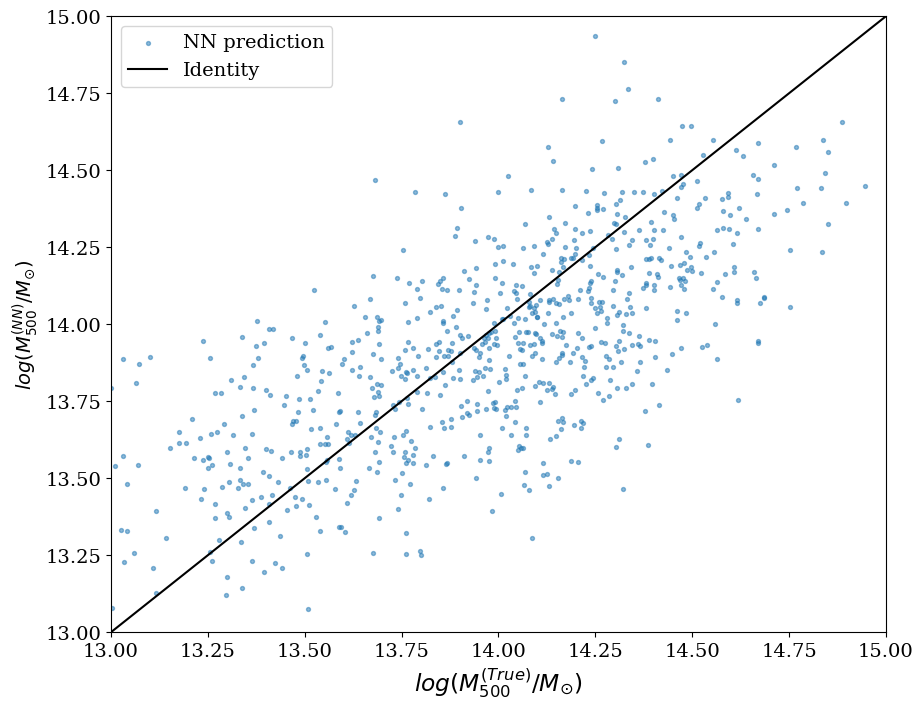
\includegraphics[width=\linewidth]{images/Chapter4/Res101/res101_test.png}
  \caption{Model predictions on the test set.}
  \label{fig:best_perf_resnet101_a}
\end{subfigure}%
\hspace{.6em}
\begin{subfigure}{.46\textwidth}
  \centering
  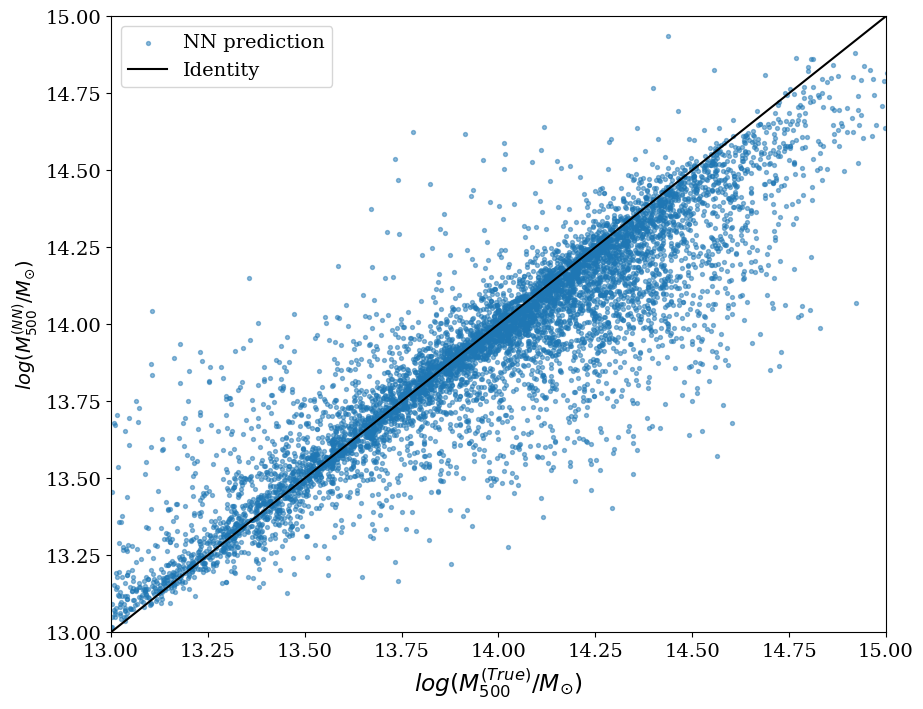
\includegraphics[width=\linewidth]{images/Chapter4/Res101/res101_train.png}
  \caption{Model predictions on the training set.}
  \label{fig:best_perf_resnet101_b}
\end{subfigure}
\begin{subfigure}{.46\textwidth}
  \centering
  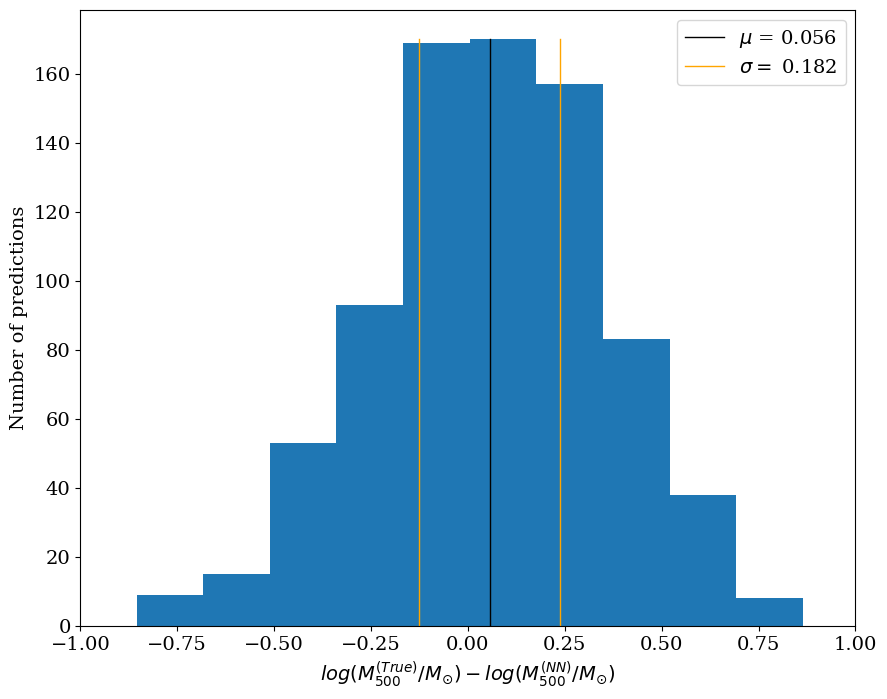
\includegraphics[width=\linewidth]{images/Chapter4/Res101/res101_test_hist.png}
  \caption{Histogram of model predictions on the test set.}
  \label{fig:best_perf_resnet101_c}
\end{subfigure}%
\hspace{.6em}
\begin{subfigure}{.46\textwidth}
  \centering
  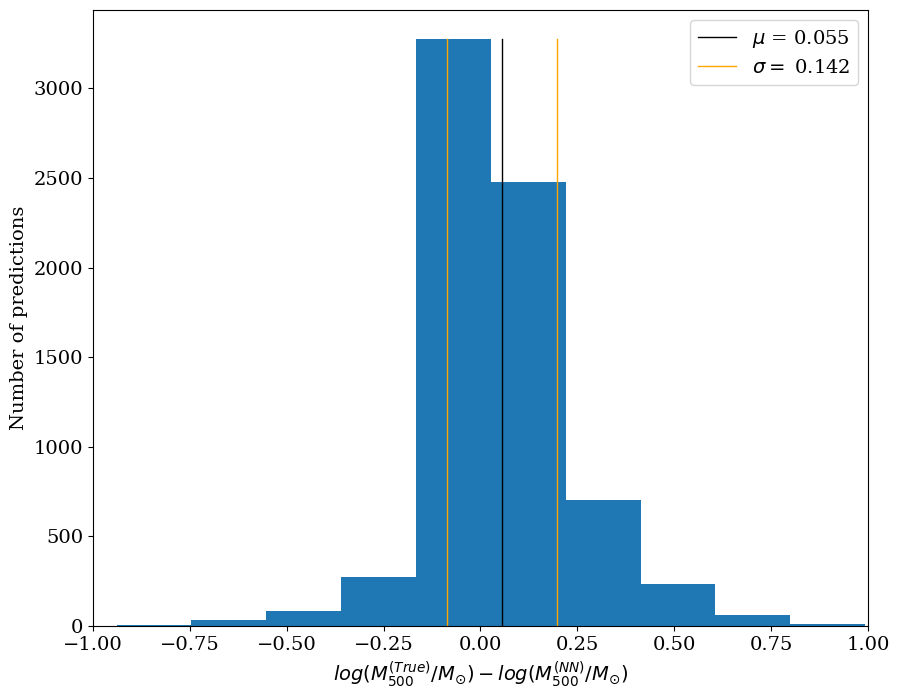
\includegraphics[width=\linewidth]{images/Chapter4/Res101/res101_train_hist.png}
  \caption{Histogram of model predictions on the training set.}
  \label{fig:best_perf_resnet101_d}
\end{subfigure}
\caption{Predictions on the training set are way better than the predictions on the test set which is a result of overfitting.} 
\label{fig:best_perf_resnet101}
\end{figure}

The overfitting can also be seen in \autoref{fig:best_perf_resnet101_a} and \autoref{fig:best_perf_resnet101_b} where the predictions on the test set are way worse than the predictions on the training set. On the other hand though, it was able to predict masses within the correct mass range, shown by the small $\mu$ compared to ResNet50V2 for instance. Overall, the performance of the ResNet101 model was not as good as other ResNet models such as ResNet50V2 and ResNet152V2 because the standard deviation of the difference between the predicted and the true mass was too high ($\sigma = 0.185$). The high variance in training also indicates that this model might not be ideal for galaxy cluster estimation, at least not without any optimization.
